\documentclass{home_assignment}
\usepackage[acronym,nogroupskip]{glossaries}
\usepackage[hidelinks]{hyperref}
\makeglossaries
\newacronym{it}{IT}{Information Technology}
\newacronym{ict}{ICT}{Information and Communication Technology}
\newacronym{gdp}{GDP}{Gross Domestic Product}
\newacronym{aws}{AWS}{Amazon Web Services}
\newacronym{gcp}{GCP}{Google Cloud Platform}
\newacronym{gea}{GEA}{Government Enterprise Architecture}
\newacronym{un}{UN}{United Nations}
\newacronym{ibm}{IBM}{International Business Machines Corporation}
\newacronym{ngo}{NGO}{Non-Governmental Organization}
\newacronym{www}{WWW}{World Wide Web}
\newacronym{ntc}{NTC}{Nepal Telecom}
\newacronym{egmp}{eGMP}{e-Governance Master Plan}
\newacronym{ftth}{FTTH}{Fiber to the Home}
\newacronym{atm}{ATM}{Automated Teller Machine}
\newacronym{abbs}{ABBS}{Any Branch Banking Service}
\newacronym{isp}{ISPs}{Internet Service Providers}
\newacronym{pan}{PAN}{Permanent Account Number}
\newacronym{g2c}{G2C}{Government to Citizen}
\newacronym{g2b}{G2B}{Government to Business}
\newacronym{g2e}{G2E}{Government to Employees}
\newacronym{g2g}{G2G}{Government to Government}
\newacronym{hlcit}{HLCIT}{High Level Commission of Information and Technology}
\newacronym{dbms}{DBMS}{Database Management System}
\newacronym{nitc}{NITC}{National Information Technology Center}
\newacronym{moest}{MoEST}{Ministry of Education, Science and Technology}
\newacronym{moic}{MoIC}{Ministry of Information and Communications}
\newacronym{moga}{MoGA}{Ministry of General Administration}
\newacronym{mof}{MoF}{Ministry of Finance}
\newacronym{eta}{ETA}{Electronic Transaction Act}   
\newacronym{itu}{ITU}{International Telecommunication Union}  
\newacronym{egdi}{EGDI}{e-Government Development Index}
\newacronym{covid}{COVID-19}{Corona Virus Disease of 2019}
\newcommand{\archi}[2]{
    \begin{figure}[H]
        \centering
        \includegraphics[width=\linewidth]{../Figures/archi-#1}
        \caption{#2}
        \label{fig:archi-$1}
    \end{figure}
}

\begin{document}
    \titlePage{Design of an AWS Architecture for Library e-Portal}{August 30, 2021}{Basanta Joshi, Ph.D.\\Dipak Poudel}   
    \pagenumbering{roman}
    \section*{Abstract}
    \phantomsection
    \addcontentsline{toc}{section}{\bfseries{Abstract}}
    With the growing field of \acrfull{it}, the entire world is shifting from on-premise services to cloud computing. The benefits of cloud computing over traditional on-premise methodologies is unmatched. As a part of the elective subject, Enterprise Computing, under the Department of Electronics and Communication Engineering, Pulchowk Campus, Institute of Engineering, this report presents a library e-Portal architecture on the cloud using \acrfull{aws}.
    \clearpage
    \tableofcontents
    \clearpage
    \phantomsection
    \addcontentsline{toc}{section}{\bfseries{List of Figures}}
    \listoffigures
    \clearpage
    \phantomsection
    \addcontentsline{toc}{section}{\bfseries{List of Abbreviations}}
    \printglossary[type=\acronymtype,nonumberlist,title={List of Abbreviations}]
    \clearpage
    \pagenumbering{arabic}
    \section{Problem Statement}
    With the advent and growth of cloud computing services, the on-premise servers and data centers are gradually becoming obsolete. There is no doubt that with growing demand of resources, and the necessity of widespread availability, most services have to switch to the cloud to sustain a positive impression on the users. One such field is the library facility that almost every campus must ensure for a well-rounded education system. Library facilities include book-lending, book-renewal, manual/report/project database and tracking of user's book-transactions. To ensure easy and faster access along with durable and secure results, such library systems are shifting to cloud, which is why this report suggests one such architecture for a library e-Portal on \acrshort{aws} cloud.
    \section{Requirement of the Architecture}
    For a functional library e-Portal, the overall architecture must be able to perform the following key functions,
    \begin{enumerate}
        \item Host static content.
        \item Host dynamic content.
        \item Store database content.
        \item Store file system content.
    \end{enumerate}
    If a basic library e-Portal was to be designed with a single instance, the \acrshort{ec2} host would perform all the tasks. However, for a properly implemented scalable, secure, durable and fast architecture, the functions are divided among different components provided as service by \acrshort{aws}.
    \begin{figure}[H]
        \centering
        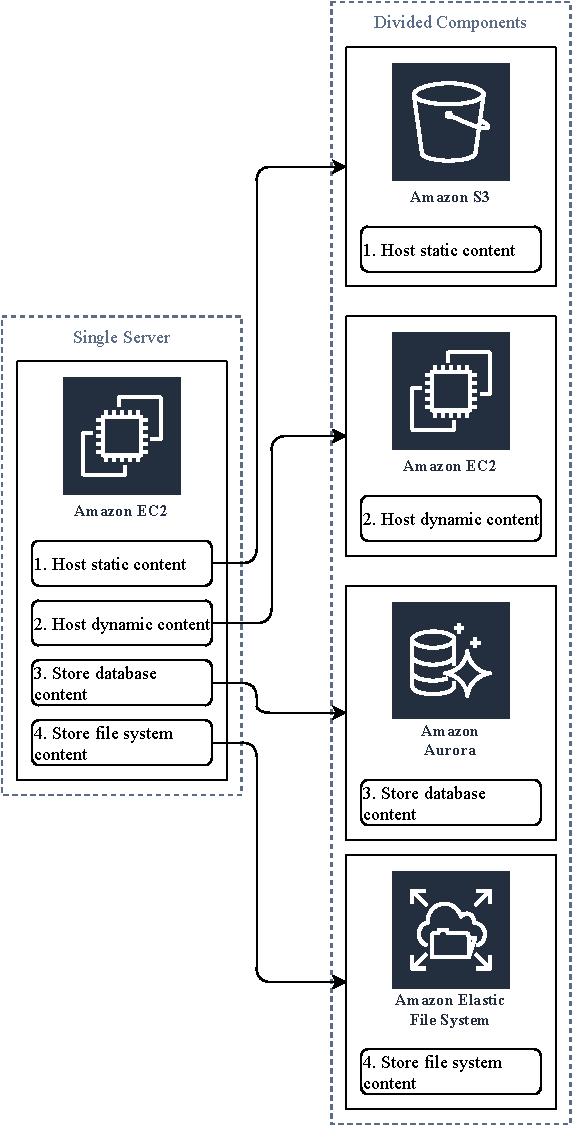
\includegraphics{../Figures/single_vs_ref}
        \caption{Single server versus divided components}
        \label{fig:single_vs_ref}
    \end{figure}
    \section{Background Theory}

    \subsection{Global Infrastructures}
    \subsubsection{AWS Cloud}
    \acrshort{aws} cloud is a group of services provided by Amazon that include \acrshort{iaas}, \acrshort{paas} and \acrshort{saas} along with different necessary components for an entire cloud architecture. In order to deliver highly reliable, scalable cloud services over a secure connection, Amazon has segregated it's global infrastructures with 81 availability zones in 25 actual global regions around the globe.
    \subsubsection{AWS Regions}
    These are physical geographical locations where data replication across regions depends on the clients need. Currently there are 25 \acrshort{aws} regions that themselves house one or more availability zones. Each region is completely independent of one another and pricing vary in these regions.
    \subsubsection{Availability Zones}
    These are isolated AWS infrastructures inside an AWS region that are connected via high bandwidth private networks. Currently there are 81 availability zones that themselves house one or more data centers. The availability zones ensure isolation from natural calamities. 21 new availability zones in 7 \acrshort{aws} regions have been announced recently.

    \subsection{Server related Services}
\subsubsection{Amazon Elastic Compute Cloud (EC2)} 
Amazon \acrfull{ec2} is a service available on the Amazon console dashboard that allows clients to create virtual machines, generally known as \acrshort{ec2} instances. In terms of cloud computing types, an \acrshort{ec2} can be regarded as an \acrshort{iaas} since the client can choose the \acrshort{ami}, and capacity of servers. The said \acrshort{ec2} instances allow clients to host virtual machines on which they can deploy applications in somewhat a similar fashion as an on-premise environment. Few use-cases where \acrshort{ec2} instances are used are as application, web, game, media, mail, database servers. \acrshort{ec2} instances can be launched in the different possible availability zones. 
\subsubsection{Elastic Load Balancing}
Elastic Load Balancing is a service provided by \acrshort{aws} that is used to distribute the incoming traffic across different target that maybe Amazon \acrshort{ec2}, \acrshort{ip} addresses, applications or Lambda functions. There are four types of \acrfull{elb}, viz. Application Load Balancer, Network Load Balancer, Classic Load Balancer and Gateway Load Balancer.
\subsubsection{Autoscaling}
Auto scaling is a service provided by \acrshort{aws} that allows users to set scaling configurations based on which various resources are scaled based on the demand requirements of the system. It is used to dynamically allocate computational resources with changing demands and helps in cost reduction, proper utilization of resources and scalability.

\subsection{Database and Storage related Services}
\subsubsection{Amazon Aurora}
\acrshort{aws} offers Amazon Aurora as a simple and cost-effective enterprise level relational database service that is also compatible with MySQL and PostgreSQL.
\subsubsection{Amazon Memcached}
Amazon Memcached is an open-source high-performance, in-memory data store used as cache store for applications on \acrshort{aws} cloud.
\subsubsection{Amazon Simple Storage Service (S3)}
Amazon \acrfull{s3} is the object storage service provided by \acrshort{aws}. Amazon promotes \acrshort{s3} as a highly scalable, available, durable (99.999999999\%) and secure object storage service. Objects are stored in \acrshort{s3} buckets that are globally unique and located in a region. 
\subsubsection{Amazon Elastic File System (EFS)}
Amazon \acrfull{efs} is a file storage system for the applications that run on \acrshort{aws}. It is used to avoid performance bottlenecks as it provides flexible storage capacity to multiple connected instances.
\subsection{Networking related Services}
    \subsubsection{Virtual Private Cloud (VPC)}
    \acrfull{vpc} is a service provided by \acrshort{aws} that allows users to create private, isolated virtual networks on the public environment essentially providing much needed isolation to different resources on \acrshort{aws}.
    \subsubsection{Subnet}
    Subnet, as the name suggests is a smaller (sub) piece of a larger network (net). Logical division of \acrshort{ip} addresses create the required ambiguity among different components of a larger system. Private subnets are those that don't have public \acrshort{ip} assigned, hence aren't directly accessible over the internet. Similarly, public subnets can be accessed over the internet.
    \subsubsection{Amazon Route 53}
    Amazon Route 53 is a \acrfull{dns} service provided by \acrshort{aws} that provides domain registration, health checking in addition to \acrshort{dns} routing.
    \subsubsection{Amazon Cloudfront}
    Amazon Cloudfront is a \acrfull{cdn} service provided by \acrshort{aws} that provides a globally distributed content delivery service using proxy servers to cache contents at various edge locations.
    \subsubsection{Internet Gateway}
    An internet gateway, as the name suggests is the gateway between a \acrshort{vpc} and the internet. It provides a target in a \acrshort{vpc} route table for the traffic and also performs \acrfull{nat} for the instances that have been assigned public \acrshort{ip} addresses. 
   \subsubsection{Network Address Translation (NAT) Gateway}
  For instances that are placed in a private subnet, a \acrfull{nat} gateway is required to connect to the internet. A \acrshort{nat} gateway provides instances in private subnets access to public internet outbound traffic while blocking incoming connections. It is essential for connecting instances to the internet during software updates or patch installations.
    \section{Library e-Portal Architecture}
    The architecture design starting from the basic setup to the final design is included as,
  \archi{1}{Basic setup with a single \acrshort{ec2} instance}
  A simple library e-Portal can be run using a single \acrshort{ec2} instance connected to an internet gateway and a working \acrshort{dns} system provided by Amazon Route53. All the work-load would be handled by the single instance and a larger system would be tedious.
  \archi{2}{Faster content delivery}
  As discussed earlier, Amazon Cloudfront is essential if the system requires best content delivery to users in different locations of the world. This not only boosts the access speed but also saves compute capacity from the instance used.
  \archi{3}{Separate database sevice}
  Since the system requires a fully-managed database, Amazon Aurora is used in a private subnet to provide additional security to the database. This allows better database management for the e-Portal and also secures the database since it will contain critical data of users.
  \archi{4}{Redundancy across availability zones}
  To avoid downtime and assure database security, a replication can be added in another availability zone. An \acrshort{elb} is required to distribute traffic to the different instances. This way the e-Portal will have better durability since a rare failure of one instance or a database wouldn't totally damage the system.
  \archi{5}{Resource utilization as per demand}
  As discussed earlier, auto-scaling enables a system to scale according to the requirements hence saving cost since the servers will be scaled down during holidays when the users won't be much active and also ensure that the service don't get overwhelmed during peak traffic such as examination time. 
  \archi{6}{Placing instances in private subnets}
  Similar to the database servers, the \acrshort{ec2} instances placed in private subnets provide additional security from malicious contents. However, the instance would not have connection to the internet hence disrupting the software updates and patch installations, which is why  \acrshort{nat} gateways are used. \acrshort{aws} suggests the use of a Bastion Host, which is a way to securely access \acrshort{ec2} instances located in a private subnet. Placing the Bastion Host inside an auto-scaling group ensures the proper scaling if traffic were to increase.
  \archi{7}{Caching for faster response time}
  Use of a cache memory system reduces the database burden and also provides faster responses making it quite useful for performance boosts. This way the database requests would have a faster response time and frequently searched queries would be cached to reduce load.
  \archi{8}{Shared file system}
  As discussed earlier, Amazon \acrshort{efs} can be used to provide a shared file system that the different \acrshort{ec2} instances can use for a shared disk space. 
  \archi{9}{Final architecture for library e-Portal}
  Lastly the static contents for the portal can be placed in a \acrshort{s3} bucket. The static objects placed in the bucket can be easily access providing an essential storage service for some reports or books, images, lecture videos and such for the portal.
\end{document}